\documentclass[xcolor=dvipsnames]{beamer}
\usetheme{Madrid}

\usepackage[italian]{babel}

\usepackage[utf8]{inputenc}

\usepackage{hyperref}
\usepackage{graphicx} % Allows including images
\usepackage{booktabs} % Allows the 

\newcommand{\R}{\mathbb{R}}
\newcommand{\Z}{\mathbb{Z}}
\newcommand{\mc}[1]{\mathcal{#1}}
\newcommand{\ii}[1]{\textit{#1}}
\newcommand{\req}[1]{\stackrel{#1}{=}}
\newcommand{\bra}[1]{\langle #1 |}
\newcommand{\ket}[1]{| #1 \rangle}
\newcommand{\braket}[2]{\langle #1 | #2 \rangle}

\title{Geometric Deep Learning}
\author{Tommaso Lamma}
\date{2021}

\begin{document}

\titlepage

\tableofcontents

\section{Introduzione}

\frame{\titlepage}

\section{Reti Convoluzionali}

\begin{frame}
    \frametitle{Reti Convoluzionali}
    \begin{figure}[H]
        \centering
        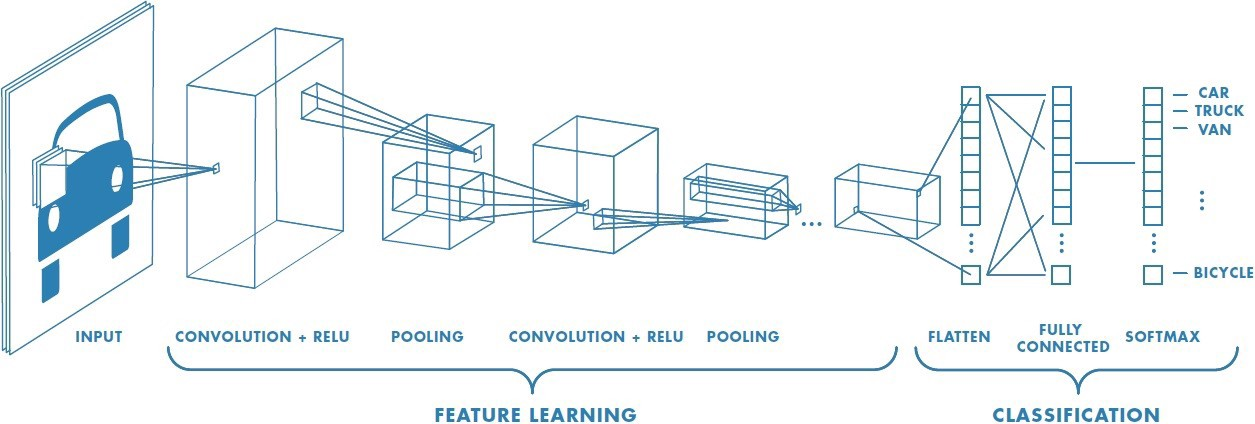
\includegraphics[width=10cm, height=4cm]{cnn}
        \caption{Una rete neurale convoluzionale.}
    \end{figure}       
\end{frame}

\section{Convoluzione su Domini Euclidei}

\begin{frame}
    \frametitle{Convoluzione su Domini Euclidei}    
    Siano $f:\R^n \to \R$ e $g:\R^n \to \R$,
    \[ (f * g)(x) = \int_{\R^n} dx' f(x')g(x-x'). \]
    \hfill \\
    \hfill \\
    { \large Cosa significa $(x - x')$ in un dominio diverso da $\R^n$ ?}
\end{frame}

\begin{frame}
    \frametitle{ \large Cosa significa $(x - x')$ \textbf{in} $\R^n$ ?}
    \hfill \\
    \hfill \\
    Possiamo vedere $( x - x')$ come l'azione dell'elemento $(-x')$ del gruppo delle traslazioni $(\R^n, +)$
    sul dominio $\R^n$(A priori della struttura di spazio vettoriale).
    \begin{block}{Notare:}
        Il gruppo $(\R^n, +)$ è una simmetria globale del dominio $\R^n$.  
    \end{block}
    \hfill \\
    \hfill \\
    {\large Possiamo definire una convoluzione su un dominio a partire dalla simmetria globale del dominio?}
\end{frame}

\begin{frame}
    \begin{figure}[H]
        \centering
        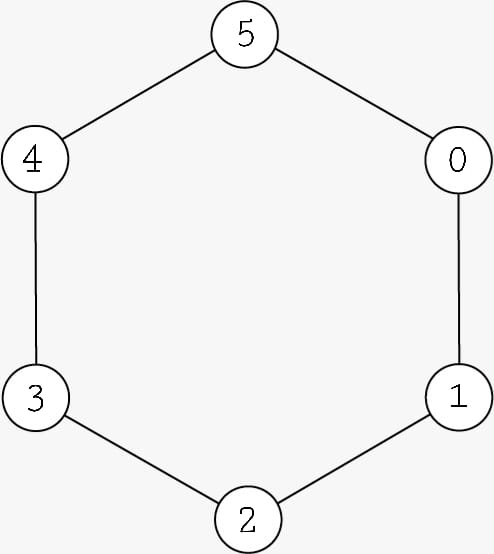
\includegraphics[width=5cm, height=5cm]{graph}
        \caption{Un dominio non euclideo $\mc{G}$.}
    \end{figure}    
\end{frame}

\begin{frame}
    \begin{block}{Spazio dei Segnali su $\mc{G}$}
        Lo spazio dei segnali a valori reali definiti su questo dominio può essere rappresentato come
        \[ \mc{S} =\{ | \psi \rangle =  \sum_{i \in \Z_6} \psi_i | i \rangle \; : \psi_i \in \R \} ,\] 
        dove devono valere 
        \[ \langle i | j \rangle = \delta_{ij}, \] 
        \[ \sum_{i \in \Z_6} | i \rangle \langle i | = \widehat{1} .\]      
    \end{block}
\end{frame}

\begin{frame}
    Una simmetria di questo spazio è il gruppo ciclico $(\Z_6,+)$ rispetto all'azione che segue.
    \begin{block}{Azione di $\Z_6$ su $\mc{S}$ }
        Un'azione di $\Z_6$ sullo spazio dei segnali è data da
        \[ . : \Z_6 \times \mc{S} \to \mc{S}\] \[ (j,| \psi \rangle) \mapsto j.| \psi \rangle = \sum_{i \in \Z_6} \psi_{i + j} | i + j \rangle \in \mc{S} .\]        
    \end{block}   
\end{frame}

\begin{frame}
Vediamo come agisce il generatore del gruppo
    \begin{block}{Azione del generatore}
        \[ 1.| \psi \rangle = \sum_{i \in \Z_6} \psi_{i + 1} | i + 1 \rangle.\]
        Le componenti trasformano nel seguente modo
        \[ \langle i | \psi \rangle =  \psi_i \mapsto \sum_{i,j \in \Z_6} S_{ij} \psi_j = \sum_{i,j \in \Z_6} \langle i | \widehat{S} | j \rangle  \langle j | \psi \rangle, \]
        dove $ S_{ij} = circ(0,1,0,0,0,0) =: \begin{pmatrix} 0 & 1 & 0 & 0 & 0 & 0 \\ 0 & 0 & 1 & 0 & 0 & 0 \\ 0 & 0 & 0 & 1 & 0 & 0
        \\ 0 & 0 & 0 & 0 & 1 & 0 \\ 0 & 0 & 0 & 0 & 0 & 1 \\ 1 & 0 & 0 & 0 & 0 & 0 \\ 
    \end{pmatrix} $.
    \end{block}    
\end{frame}

\section{Convoluzione Spettrale}

\begin{frame}
    \frametitle{Convoluzione Spettrale}
    Data la simmetria avremo che per qualsiasi osservabile $\widehat{O}$
    \[ [\widehat{S}, \widehat{O}] = 0 . \]
    L'operatore $\widehat{S}$ è diagonalizzabile $\widehat{S} |s_i \rangle = s_i | s_i \rangle$ in $\C$,\\ sfruttando l'analogia con $\R^n$ otteniamo una trasformata.
    \begin{block}{Trasformata di Fourier in $\mc{S}$}
        \[ \langle i | \psi \rangle \mapsto \langle s_i | \psi \rangle. \]
    \end{block}
    Dalla traformata definiamo per le componenti una convoluzione in analogia con $\R^n$.
    \begin{block}{Convoluzione su $\mc{S}$}
        \[ \langle s_i | \psi * \phi \rangle = \langle s_i | \psi \rangle \langle s_i | \phi \rangle . \]
    \end{block}   
\end{frame}

\section{Convoluzione Equivariante}

\begin{frame}
    \frametitle{Convoluzione Equivariante}
    Sia $\widehat{C}_\phi | \psi \rangle = | \psi * \phi \rangle$, possiamo decidere di definire questa convoluzione solo a partire da
    \[ [\widehat{S}, \widehat{C}_\phi] = 0, \]
    ciò implica che la matrice associata a $\widehat{C}_\phi$ è circolante.

    \begin{block}{Notare:}
        In entrambi i casi abbiamo ridotto il numero di parametri \\ da imparare da \textbf{36} a \textbf{6}.
    \end{block}
\end{frame}






\end{document}